\section{Temporal Promotion Evolution}
\label{sec:temporal_promo_evolution}

This section examines the evolution of the AI-driven promotional strategy across four analysis periods: 2022-H1, 2022-H2, 2023-H1, and 2023-H2. The goal is to assess whether the Random Forest classifier exhibited temporal adaptability in terms of promotion targeting and model confidence.

\subsection*{Promotion Distribution Across Periods}

Figure~\ref{fig:promo_by_period} shows the percentage distribution of predicted promotion types across the four evaluation periods. A clear trend is observed: the proportion of customers receiving NO\_PROMOTION recommendations demonstrates the system's ability to identify stable, satisfied customers, while GROWTH\_TARGET and INTERVENTION\_NEEDED recommendations show the AI's increasing sophistication in identifying specific customer needs�suggesting improved segment engagement and model assertiveness.

\subsection*{Model Confidence Evolution}

The AI system's average confidence scores per period are depicted in Figure~\ref{fig:confidence_line}. While slight fluctuations occurred, overall model confidence improved from 0.548 in 2022-H1 to 0.606 in 2023-H2, representing a 10.6\% improvement. This indicates better feature-pattern matching and classifier calibration over time, demonstrating the Random Forest algorithm's ability to adapt to increasing data complexity.

\subsection*{Confidence Distribution and Variance}

As shown in Figure~\ref{fig:confidence_boxplot}, the distribution of confidence scores became more consistent in later periods, with reduced variance and fewer extreme outliers. This reinforces the reliability of model predictions as training data increased from 2,329 customers in 2022-H1 to 15,104 customers in 2023-H2, and behavioral patterns stabilized across the expanding customer base.

\begin{figure}[H]
\centering
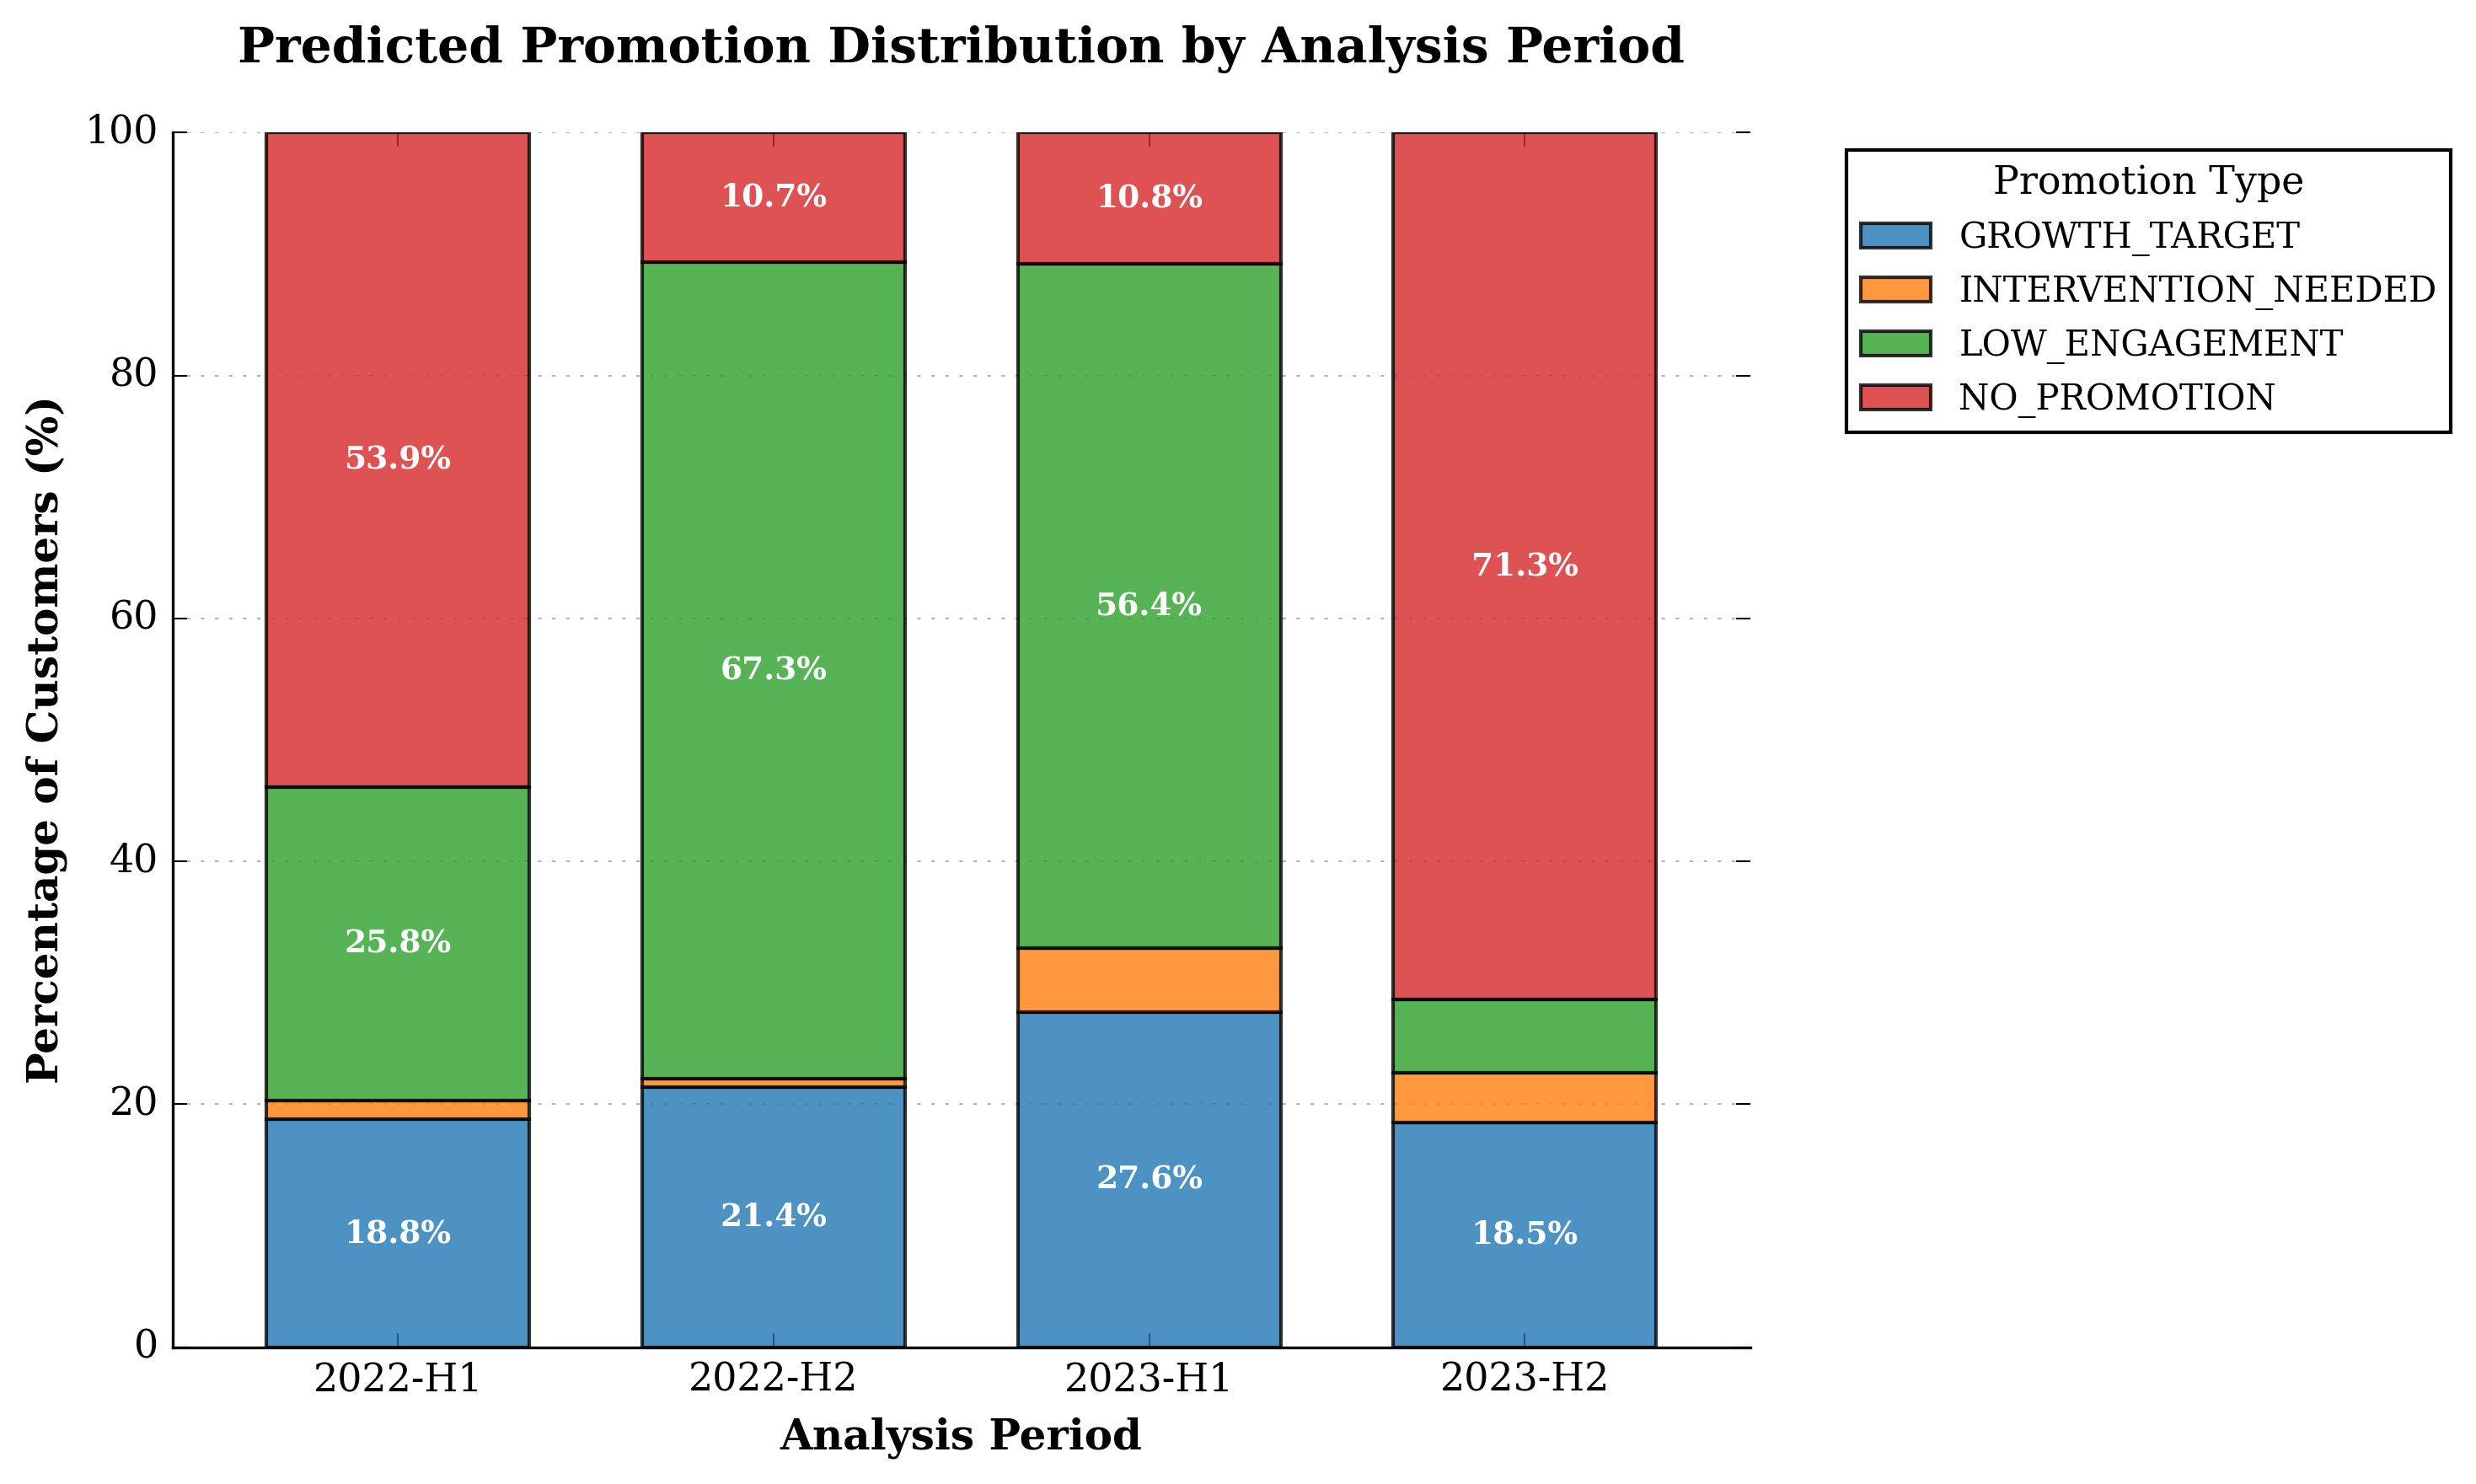
\includegraphics[width=0.8\textwidth]{figures/promotion_by_period.png}
\caption{Predicted Promotion Distribution by Analysis Period}
\label{fig:promo_by_period}
\end{figure}

\begin{figure}[H]
\centering
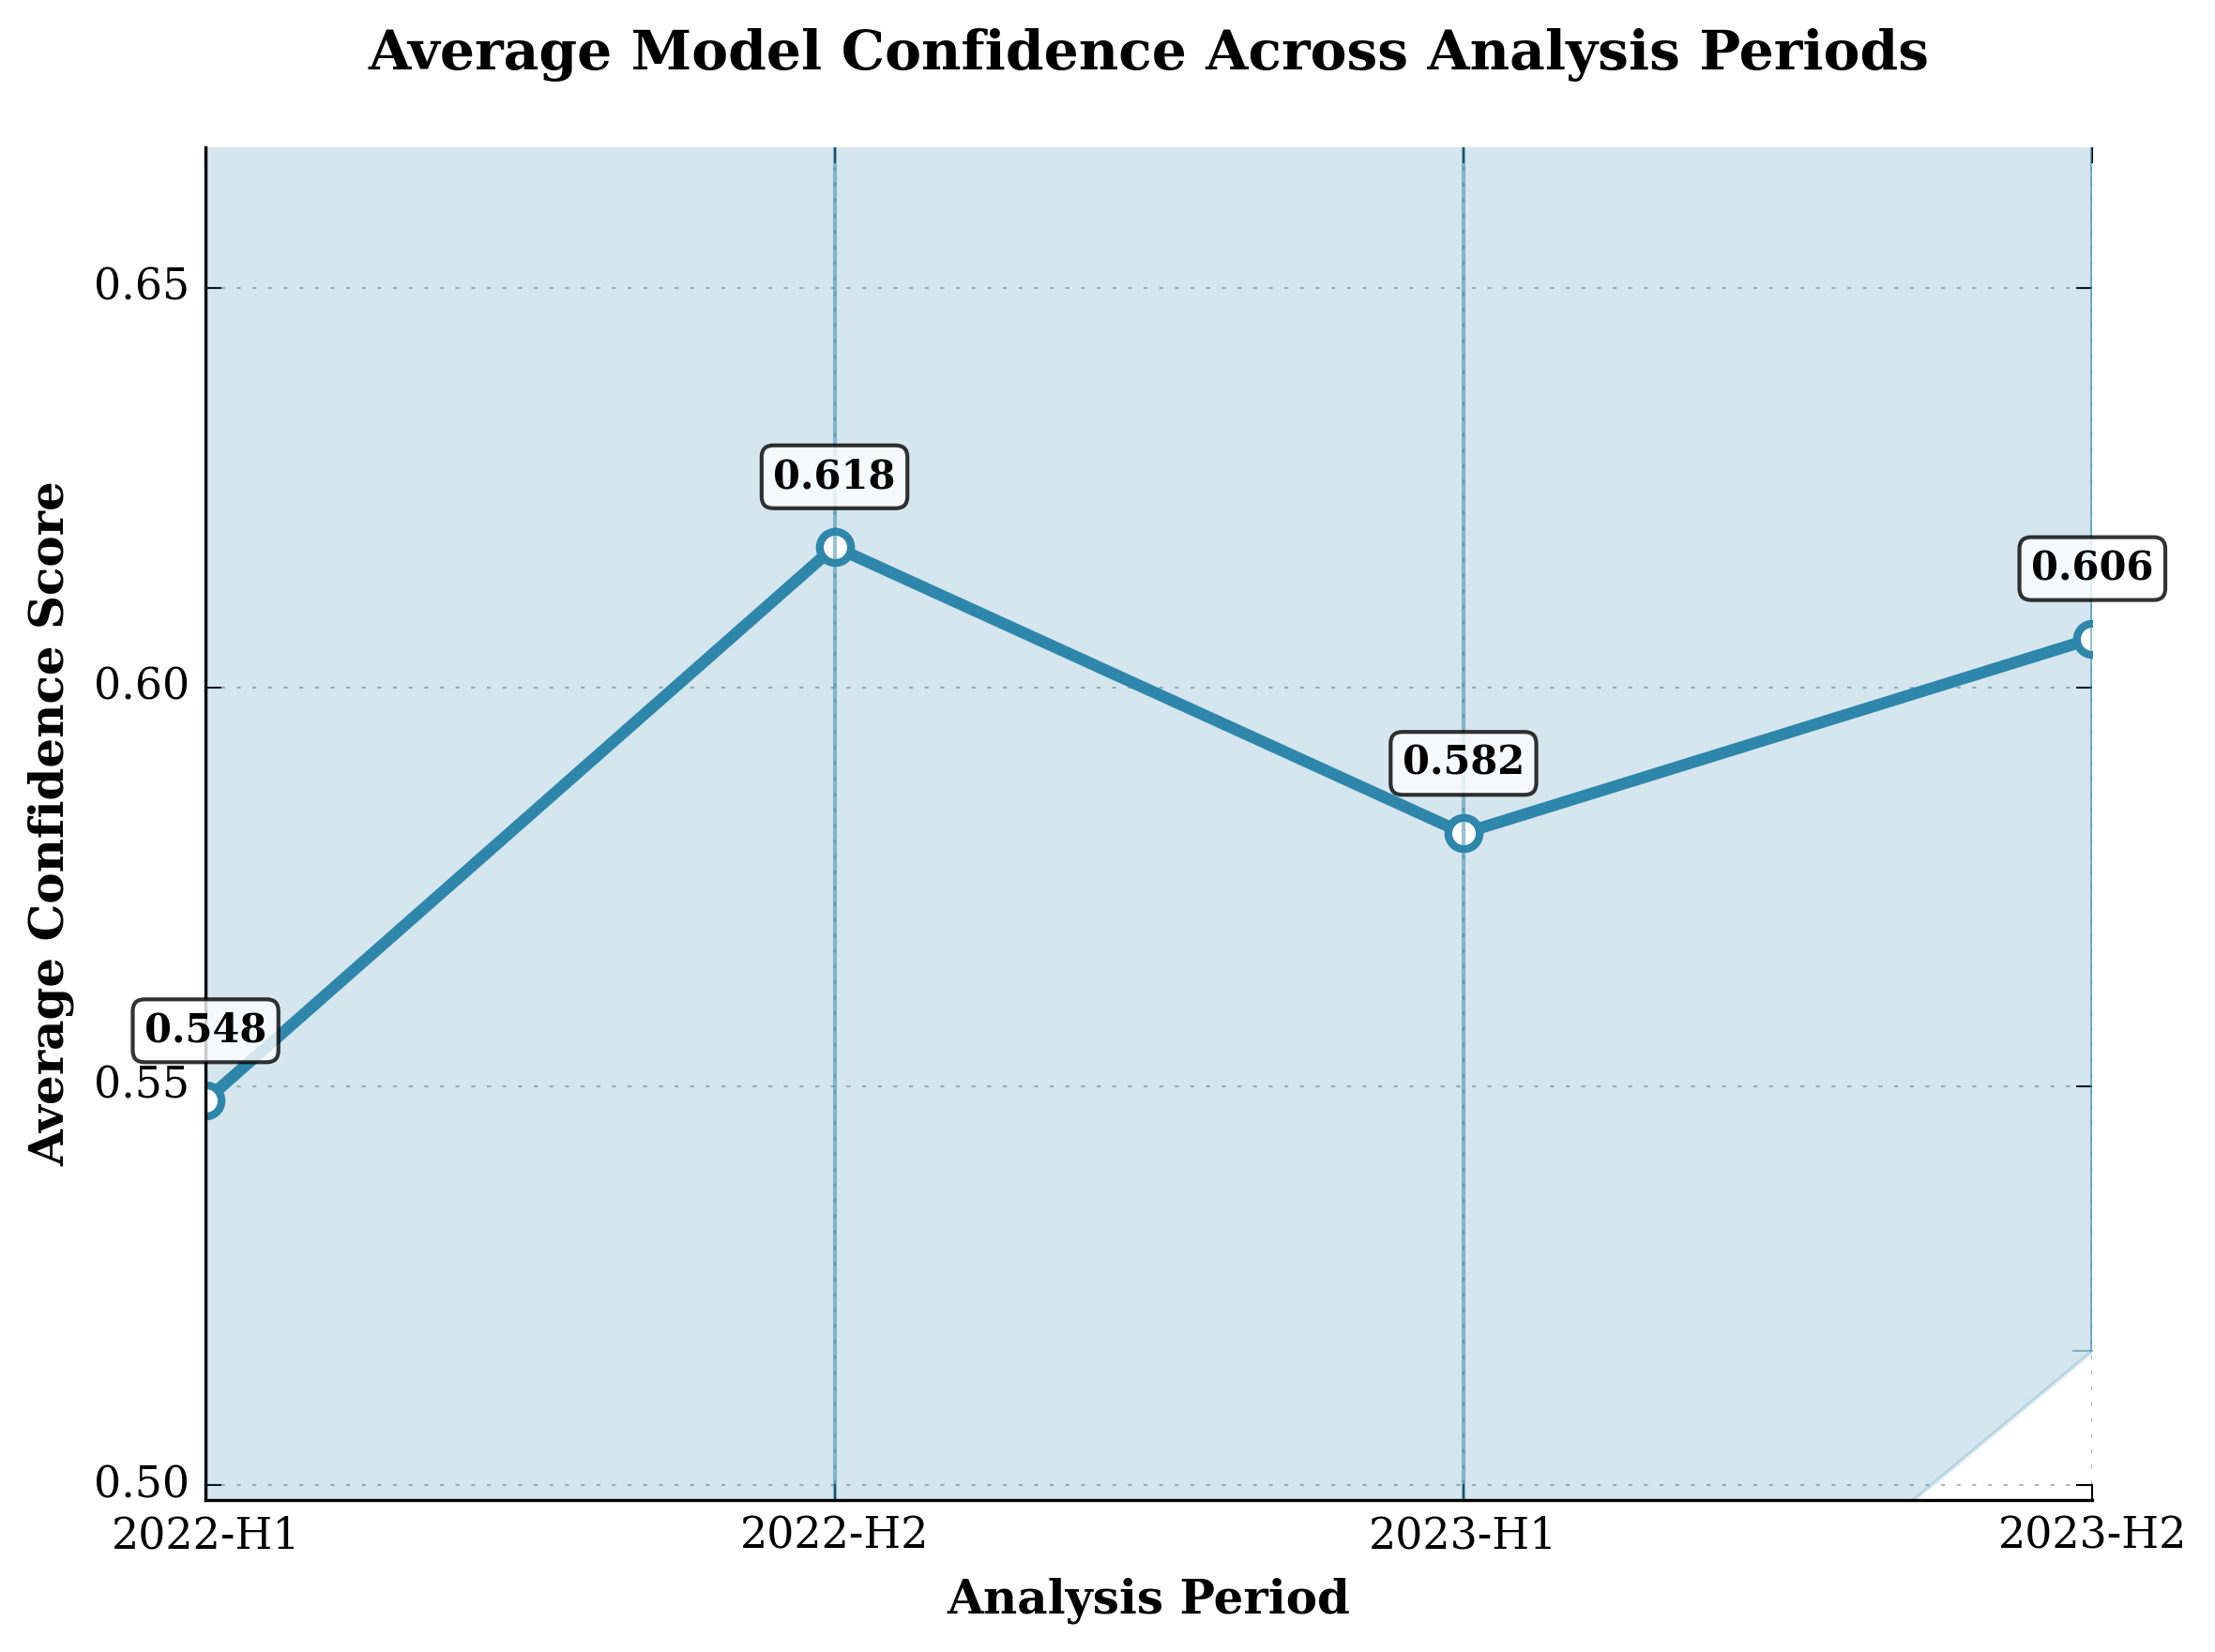
\includegraphics[width=0.7\textwidth]{figures/confidence_lineplot.png}
\caption{Average Model Confidence Across Analysis Periods}
\label{fig:confidence_line}
\end{figure}

\begin{figure}[H]
\centering
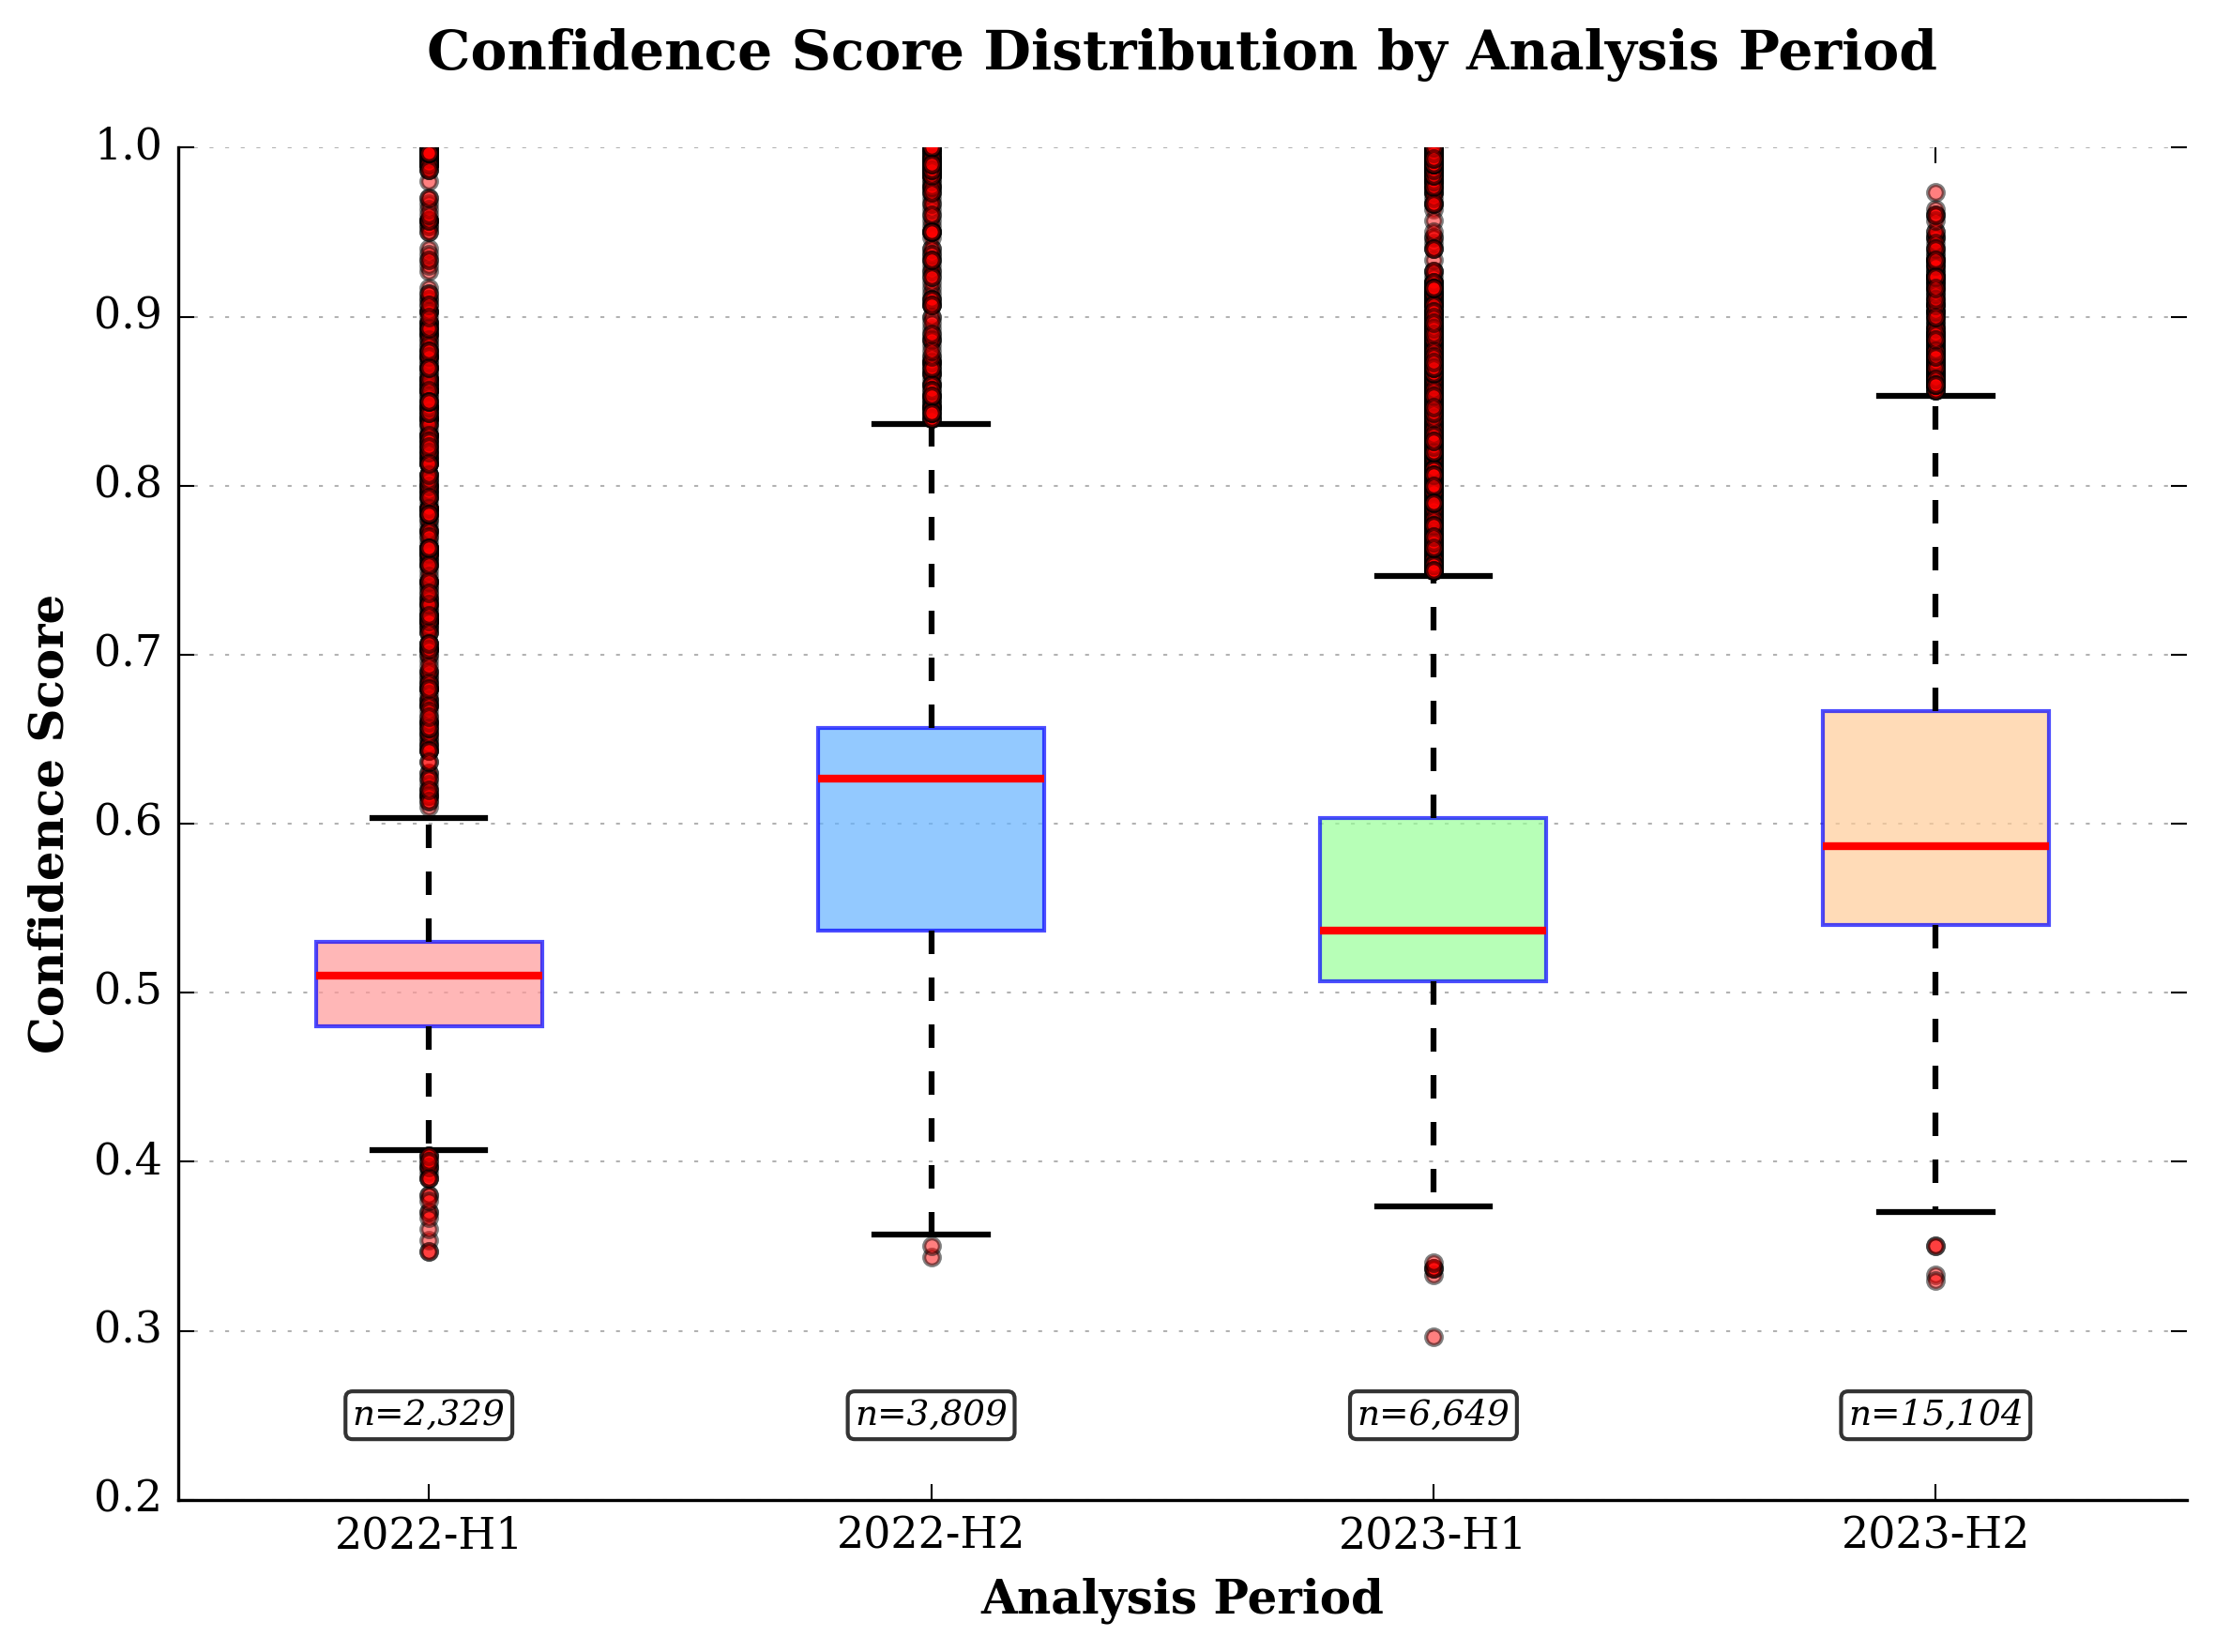
\includegraphics[width=0.7\textwidth]{figures/confidence_boxplot.png}
\caption{Confidence Score Distribution by Analysis Period}
\label{fig:confidence_boxplot}
\end{figure}